\documentclass[12pt,oneside,a4paper]{article}
\usepackage{amsmath}
\usepackage{tabularx}
\usepackage{graphicx}
\usepackage[hidelinks]{hyperref}
\usepackage[top=1.2in]{geometry}
\usepackage{abstract}
\usepackage{setspace}
\usepackage{enumitem}
\usepackage[nodayofweek]{datetime}
\usepackage{cite}
\usepackage{times}
\usepackage{ragged2e}

%%%%%%%%%%%%%%%%%%%%%%%%%%%%%%%%%%%%%%%%%%%%%%%%%%%%%%%%%%%%%%%%%%%%%%%

\usepackage[table]{xcolor}
\usepackage{pdfpages}


\usepackage{natbib}
\usepackage{bibentry}
\nobibliography*

%%%%%%%%%%%%%%%%%%%%%%%%%%%%%%%%%%%%%%%%%%%%%%%%%%%%%%%%%%%%%%%%%%%%%%%

\usepackage{lipsum}

\newcommand\todo[1]{\textcolor{blue}{#1}}
\newcommand\placeholder[1]{\todo{\lipsum[#1]}}

%%%%%%%%%%%%%%%%%%%%%%%%%%%%%%%%%%%%%%%%%%%%%%%%%%%%%%%%%%%%%%%%%%%%%%%

\definecolor{Green}{rgb}{0,0.7,0.1}

\providecommand\phantomsection{}

\tolerance=1
\emergencystretch=\maxdimen
\hyphenpenalty=10000
\hbadness=10000

\renewcommand{\abstractnamefont}{\normalfont\Large\bfseries}

\title{{\huge{IDENTIFY BLOOM KNOWLEDGE OF STUDENT}} \\ [30pt]
	\large{MINI PROJECT REPORT \\ SUBMITTED TO \\ [30pt] RAMAIAH INSTITUTE OF TECHNOLOGY} \\
	\normalsize{(Autonomous Institute, Affiliated to VTU)} \\ [10pt]
	\large{Bangalore - 560054} \\ [25pt]
	\normalsize\textsc{Submitted by} \\ [10pt]
	\begin{minipage}{0.6\textwidth}
		M Sneha \hfill 1MS14CS058 \\
		Mipsa Patel \hfill 1MS14CS148 \\
		Tilak S Naik \hfill 1MS14CS134 \\
		Vibha Karanth \hfill 1MS14CS136
	\end{minipage} \\ [30pt]
	\normalsize{As part of the Course \textbf{Data Analytics Laboratory - CSL717}} \\ [20pt]
	\large\textsc{SUPERVISED BY} \\
	\textbf{Parkavi. A} \\ \vfill
	
\includegraphics{rit.png} \\ [15pt]
	\large{DEPARTMENT OF COMPUTER SCIENCE \& ENGINEERING} \\ [5pt]
	RAMAIAH INSTITUTE OF TECHNOLOGY \\ [5pt]
	\large{Sep - Dec 2017}
	\thispagestyle{empty}
	\newpage
	Department of Computer Science and Engineering \\ [10pt]
	Ramaiah Institute of Technology \\
	\normalsize{(Autonomous Institute, Affiliated to VTU)} \\ [10pt]
	\large{Bangalore - 54} \\ [30pt]
	
\includegraphics{rit.png} \\ [20pt]
	\Large\textbf{CERTIFICATE} \\ [40pt]
	\normalsize \justify This is to certify that M Sneha (1MS14CS058), Mipsa Patel (1MS14CS148), Tilak S Naik (1MS14CS134), Vibha Karanth (1MS14CS136) have completed ``Identify Bloom Knowledge of Student'' as part of Mini Project. \\ [10pt]
We declare that the entire content embodied in this B.E. 7th Semester report contents are not copied. \\
	\vspace{\fill}
	\makebox[\textwidth]{
		\begin{minipage}{.4\textwidth}
			Submitted by \\ [10pt]
			M Sneha \hfill 1MS14CS058 \\
			Mipsa Patel \hfill 1MS14CS148 \\
			Tilak S Naik \hfill 1MS14CS134 \\
			Vibha Karanth \hfill 1MS14CS136 \\ [10pt]
			(Dept of CSE, RIT)
		\end{minipage}
		\hfill
		\begin{minipage}{.4\textwidth}
			\centering
			Guided by \\ [10pt]
			Prof. Parkavi \\
			Assistant Professor \\
			(Dept. of CSE, RIT)
		\end{minipage} \\
	}
}

\author{}
\date{}

\begin{document}
	\maketitle
	\thispagestyle{empty}
	\newpage
	\thispagestyle{empty}
	
	\centering
	Department of Computer Science and Engineering \\ [10pt]
	Ramaiah Institute of Technology \\
	\normalsize{(Autonomous Institute, Affiliated to VTU)} \\ [10pt]
	\large{Bangalore - 54} \\ [30pt]
	
\includegraphics{rit.png} \\ [10pt]
	\textbf{\underline{Evaluation Sheet}} \\ [20pt]
	\small
	\vspace{\fill}
	{\renewcommand{\arraystretch}{1.75}
		\begin{tabular}{|m{0.25cm}|>{\centering\arraybackslash}m{2cm}|>{\centering\arraybackslash}m{2.25cm}|>{\centering\arraybackslash}m{1.1cm}|>{\centering\arraybackslash}m{0.8cm}|>{\centering\arraybackslash}m{0.6cm}|>{\centering\arraybackslash}m{0.6cm}|>{\centering\arraybackslash}m{1cm}|>{\columncolor[HTML]{AAEDAC}}m{1cm}|}
			\hline
			 \textbf{Sl. No} & \textbf{USN} & \textbf{Name} & \textbf{Content and Demon-stration (15)} & \textbf{Speak-ing Skills (2)} & \textbf{Team work (2)} & \textbf{Neat-ness and care (2)} & \textbf{Effect-iveness \& Produc-tivity (4)} & \textbf{Total Marks (25)} \\
			\hline
			1 & 1MS14CS058 & M Sneha &&&&&&\\
			\hline
			2 & 1MS14CS148 & Mipsa Patel &&&&&&\\
			\hline
			3 & 1MS14CS134 & Tilak S Naik &&&&&&\\
			\hline
			4 & 1MS14CS136 & Vibha Karanth &&&&&&\\
			\hline
		\end{tabular}
	} \\
	\vspace{\fill}
	\normalsize
	\justifying
	Evaluated by \\ [10pt]
	\indent \indent
	\begin{minipage}{0.4\textwidth}
		Name: Parkavi. A \\
		Designation: Assistant Professor \\
		Department: Computer Science \& Engineering, RIT \\
		Signature:
	\end{minipage} \\
	\null \hfill HOD, CSE
	\newpage
	\thispagestyle{empty}
	\tableofcontents
	\newpage
	\pagenumbering{arabic}

	\null
	\vspace{\fill}

	\phantomsection
	\addcontentsline{toc}{section}{Abstract}
	\begin{abstract}
		\normalsize
		\doublespacing
		Each student has a different set of skills and strengths that they excel in. Their level of understanding, in different concepts taught to them, varies. It is important to identify their level of understanding, and one such metric to do so is Bloom's Taxonomy of Learning Domains. Based on a student's performance in questions belonging to different Bloom's levels, he is classified into one of them. Identification of the cognitive domain of a student's learning can help in improving his skills from one of the lower levels to higher levels that rely more on complex and abstract mental ability.
	\end{abstract}

	\vspace{\fill}
	\null
	\newpage

	\section{Introduction}
		Bloom's Taxonomy of Learning Domains identifies six levels within the cognitive domain, which are Knowledge, Comprehension, Application, Analysis, Synthesis, and Evaluation. These domains range from the simple recall or recognition of facts, as the lowest level called knowledge, through increasingly more complex and abstract mental levels, to the highest order which is classified as evaluation. \\
		\\
		Given a set of questions that aim at evaluating the abilities of students in different learning domains, this project determines which level the students are best at. Two classifiers based on Na\"ive Bayes and Support Vector Machines are used to classify the students' marks into one of the levels, and the accuracy obtained using these models is compared. \\
		\\
		Na\"ive Bayes comes under the class of generative models for classification. It models the posterior probability from the class conditional densities. So the output is a probability of belonging to a class. \\
		\\
		SVM, on the other hand, is based on a discriminant function given by $y = w \cdot x+b$. Here the weights $w$ and bias parameter $b$ are estimated from the training data. It tries to find a hyperplane that maximises the margin and there is optimization function in this regard. \\
		\\
		With regard to performance, SVMs using the radial basis function kernel are more likely to perform better as they can handle the nonlinearities in the data. Na\"ive Bayes performs well when the features are independent of each other which does not always happen in real life, but it performs well even with a dependent feature set.


	\section{Literature Survey}

		\begin{description}[style=nextline]
			\item[\cite{ref:omar:2012} \bibentry{ref:omar:2012}]
			This paper proposes an automated analysis of the exam questions to determine the appropriate category based on this taxonomy. This rule-based approach applies Natural Language Processing (NLP) techniques to identify important keywords and verbs, which may assist in the identification of the category of a question. \\ 
			\newpage

			\item[\cite{ref:lekha} \bibentry{ref:lekha}]
			In this paper, a novel learning method, Support Vector Machine (SVM), is applied on different data (Diabetes data, Heart Data, Satellite Data and Shuttle data) which have two or multiclass. SVM method does not suffer the limitations of data dimensionality and limited samples. It can be seen that the choice of the kernel function and best value of parameters for the particular kernel is critical for a given amount of data. \\

			\item[\cite{ref:awad:2004} \bibentry{ref:awad:2004}]
			This paper proposes a new approach for enhancing the training process of SVM when dealing with large datasets. It is based on the combination of SVM and clustering analysis. The idea is as follows: SVM computes the maximal margin separating data points; hence, only those patterns closest to the margin can affect the computations of that margin, while other points can be discarded without affecting the final result. \\

			\item[\cite{ref:lowd:2005} \bibentry{ref:lowd:2005}]
			This paper proposes Na\"ive Bayes models as an alternative to Bayesian networks for general probability estimation tasks. Experiments on a large number of datasets show that the two take a similar time to learn and are similarly accurate, but Na\"ive Bayes inference is orders of magnitude faster. \\
		\end{description}
		
		\section{Algorithm}
		
			\subsection{Na\"ive Bayes}
				
$D$: set of tuples \\
Each tuple is an $n$ dimensional attribute vector \\
$X$: $(x_1, x_2, x_3, \dots, x_n)$ \\
Let there be $m$ classes: $C_1, C_2, C_3, \dots, C_m$ \\
Na\"ive Bayes classifier predicts $X$ belongs to Class $C_i$ iff \\
$P(C_i \mid X) > P(C_j \mid X) \text{ for } 1 \le j \le m, j \neq i$ \\
Maximum Posteriori Hypothesis: \\
$$P(C_i \mid X) = \frac{P(X \mid C_i) P(C_i)}{P(X)}$$
Maximize $P(X \mid C_i) P(C_i)$ as $P(X)$ is constant \\ [10pt]
With many attributes, it is computationally expensive to evaluate $P(X \mid C_i)$ \\ [10pt]
Na\"ive Assumption of ``class conditional independence'': \\
$$P(X \mid C_i) = \prod_k P(x_k \mid C_i)$$ \\
The different Na\"ive Bayes classifiers differ mainly by the assumptions they make regarding the distribution of $P(x_k | C_i).$
			
			\subsection{Support Vector Machine}
		
Training dataset of $n$ points - $(\vec x_1, y_1), \dots, (\vec x_n, y_n)$ \\ [10pt]
When the data is linearly separable, we use the \emph{Hard-margin} to get the separating hyperplane using 2 parallel hyperplanes that separate the data: \\
$$\vec w \cdot \vec x - b = 1$$ and $$\vec w \cdot \vec x - b = -1$$ \\
To maximize distance between two planes, ${\|\vec w\|}$ in ${\dfrac{2}{\|\vec w\|}}$ is minimized. \\ [10pt]
To prevent data points from falling into the margin, add the constraint:
$$y_{i}(\vec w \cdot \vec x_i - b) \ge 1, \text{ for all } 1 \le i \le n$$
$\vec w$ and $b$ that solve this problem determine the classifier, $\vec x \mapsto \operatorname{sgn}(\vec w\cdot \vec x - b)$.

		
		\section{Implementation}
			The following 2 pages show an IPython Notebook that uses the algorithms.
			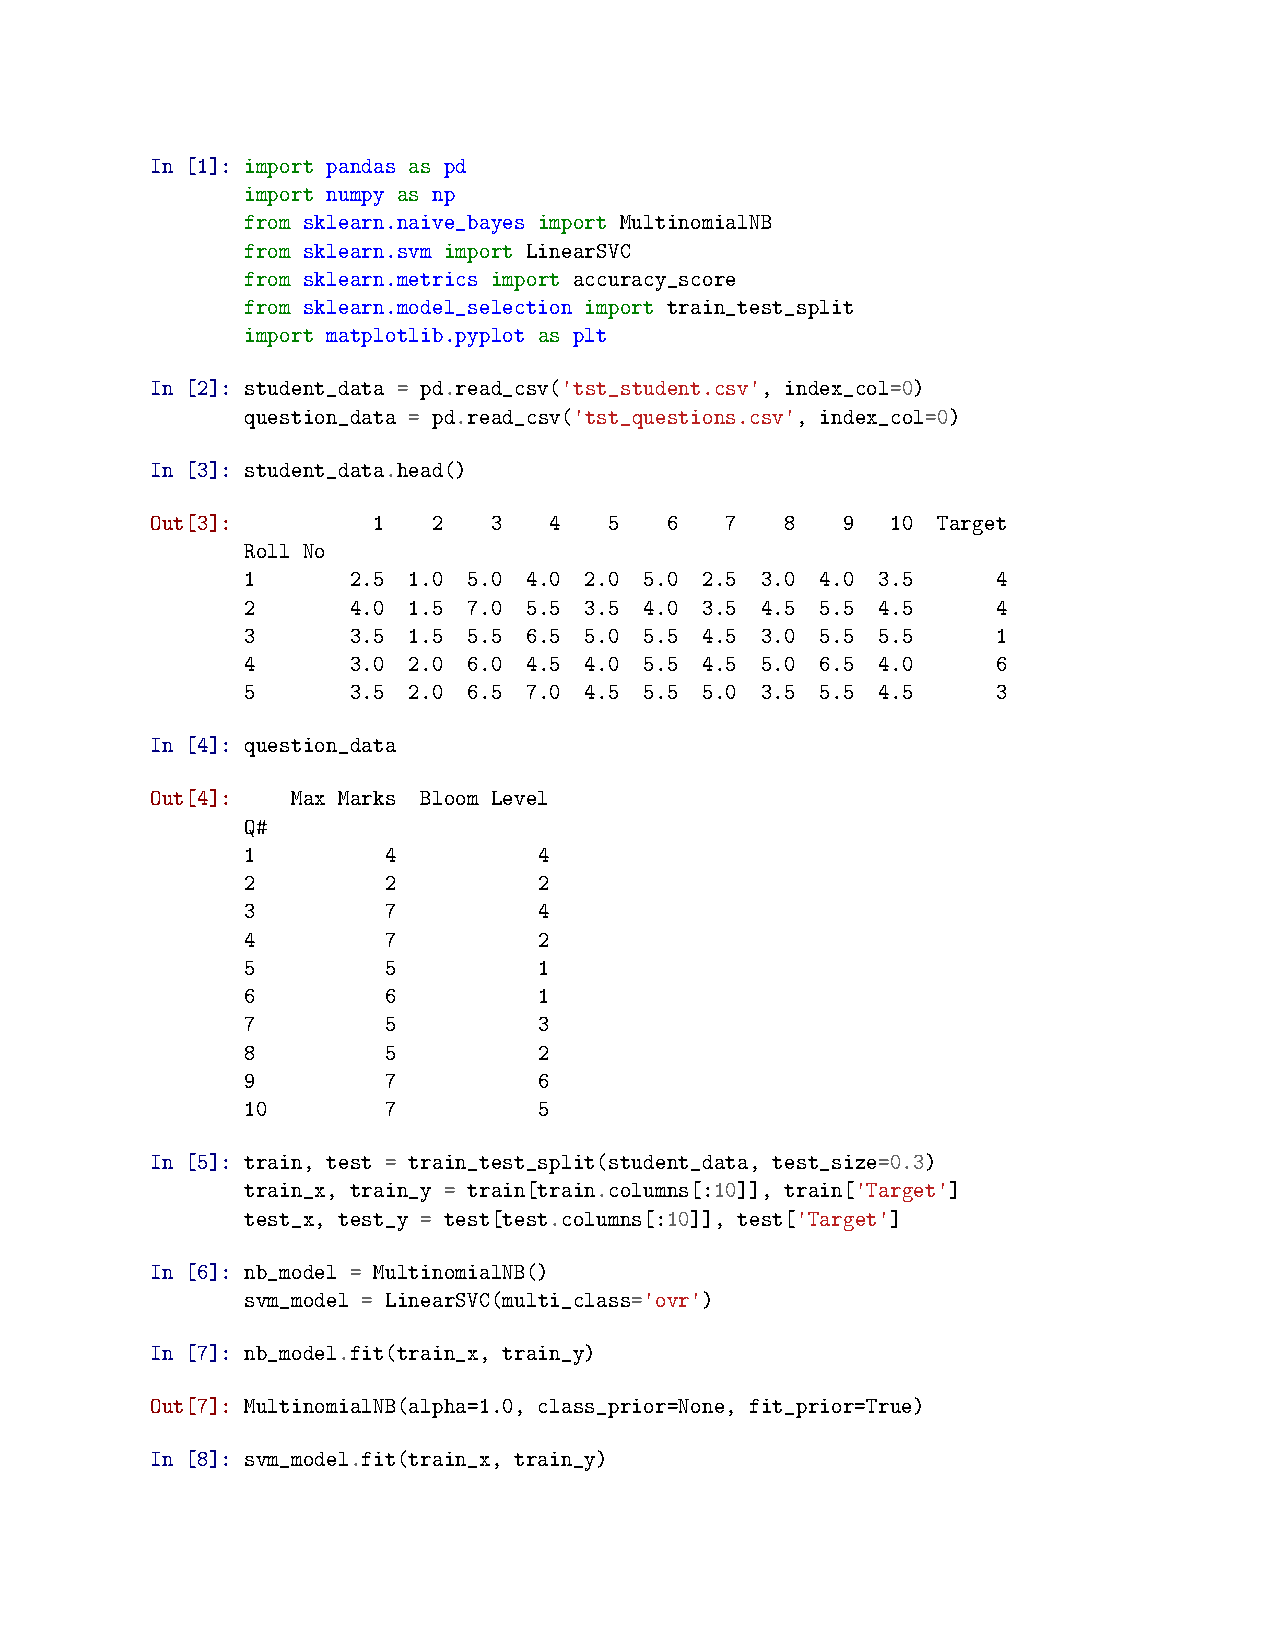
\includepdf[pages=-]{BloomLevelPredictor.pdf}
		
		\section{Results and Discussions}
		
		Na\"ive Bayes classifier gives an accuracy of $\approx 46\%$ without normalization and $\approx 30\%$ with normalization. We observe that the accuracy of the Na\"ive Bayes model does not increase significantly even by increasing the size of the dataset used to train the model. \\
		\\
		Comparatively, a model based on Support Vector Machines to obtain the Bloom's level of a student gives an accuracy of $\approx 88\%$. \\
		\\
		A comparison for prediction on 20 student's data is shown in \autoref{fig:plot}.
		
		\begin{figure}[htp]
			\centering
			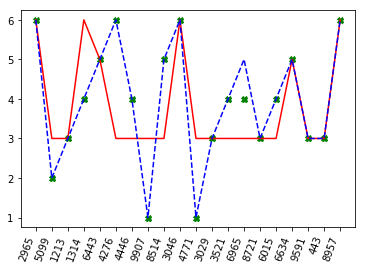
\includegraphics[scale=0.7]{BloomLevelPredictor.png}
			\caption{\small{The plot of Student ID vs Bloom Knowledge for 20 students is shown. The green crosses indicate the actual target, the red solid lines indicate the predictions by Na\"ive Bayes algorithm, and the blue dashed lines indicate the predictions by SVM.}}
			\label{fig:plot}
		\end{figure}

		\section{Conclusion}
			Classification problems can be solved using various different approaches. In this project, we explore the use of two such algorithms. Na\"ive Bayes algorithm gives a low accuracy in identification of Bloom's level. If we normalize before learning, the accuracy drops further. Support Vector Machine gives us a fairly good accuracy.

	\newpage
	\bibliographystyle{unsrt}
	\addcontentsline{toc}{section}{References}
	\bibliography{report}{}
\end{document}